% -*- root: ../main.tex -*-

% In questa sezione devono essere chiariti i compiti svolti da ciascun candidato nel caso in cui il gruppo abbia più di un componente. Deve essere inoltre esposto il piano di lavoro adottato. A tal fine, per ogni attività svolta durante la preparazione dell'elaborato (ad esempio: studio di una tecnologia, progettazione di un componente, implementazione di un algoritmo ecc. . . ) deve essere chiarita la collocazione temporale e devono essere indicate le risorse impiegate per svolgerla (giorni/uomo). I candidati possono ricorrere a opportuni diagrammi come quello di Gantt.
% 2000 - 4000 battute

\chapter{Piano di lavoro}
Il lavoro è stato svolto utilizzando un approccio Scrum, con quattro sprint, più uno iniziale incentrato sullo studio delle tecnologie.
\section{Contributi}
Di seguito vi è una descrizione delle mansioni che sono state svolte dai membri del gruppo.
\paragraph{Sara Kiade} 
\begin{itemize}
    \item progettazione e realizzazione del database
    \item implementazione logiche di interrogazione e calcolo nel back-end della Web-App
    \item implementazione e testing delle funzioni nel front end 
    \item stesura template delle funzioni nel back-end
    \item configurazione SAM
    \item prototyping della sensoristica
    \item realizzazione diagrammi sequenza
\end{itemize}

\paragraph{Gyordan Caminati}
\begin{itemize}
    \item implementazione del front-end
    \item integrazione nelle adeguate pagine del front-end delle chiamate al backend 
    \item configurazione SAM
    \item implementazione di alcune funzioni nel backend
    \item scheduling di funzioni lambda innescate da Crono Cloud Watch, MQTT, Api Gateway
    \item implementazione scheduler Micropython
    \item prototyping della sensoristica
    \item realizzazione diagrammi sequenza
\end{itemize}
\paragraph{Igor Lirussi}
\begin{itemize}
    \item implementazione scheduler Micropython
    \item implementazione funzioni core di Micropython e classi per sensori/attuatori
    \item implementazione sistema di videosorveglianza con motion detecion e object detection
    \item implementazione script di automatizzazione caricamento file
    \item prototyping della sensoristica
    \item progettazione e implementazione macchina a stati 
\end{itemize}
La collocazione temporale degli sprint è descritta nel seguente diagramma di Gantt: 
\begin{figure}[H]
    \caption{Gantt Chart del progetto}
    \label{fig:Gantt}
    \centering
   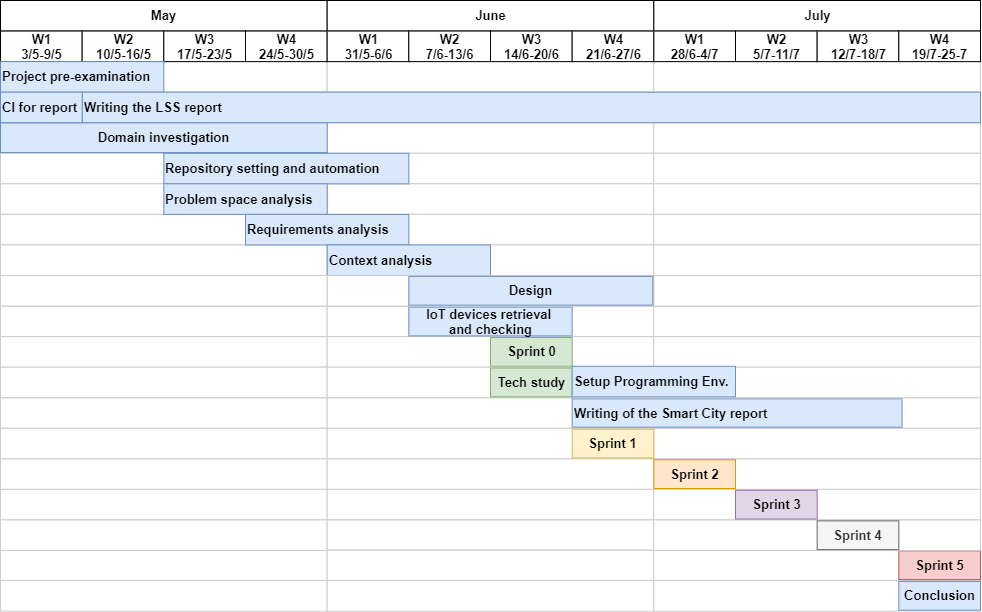
\includegraphics[width=1\textwidth]{DrawIo/GanttChart.png}
\end{figure}